% The generic preamble
\documentclass[10pt,letterpaper,fleqn,titlepage]{article}

% Define packages to use
\usepackage{natbib}
\usepackage[dvips]{graphicx,color}
\usepackage{amsmath,amssymb}
\usepackage{bm}
\usepackage{caption}
\usepackage{xr}
\usepackage{ifthen}
\usepackage[dvipdfm,colorlinks,linkcolor=blue,citecolor=blue,urlcolor=blue]{hyperref}
\usepackage{fancybox}
\usepackage{textcomp}
\usepackage{alltt}
%\usepackage{floatflt}
%\usepackage{svn}


% Redefine default page
\setlength{\textheight}{9in}  % 1" above and below
\setlength{\textwidth}{6.75in}   % 0.5" left and right
\setlength{\oddsidemargin}{-0.25in}

% Redefine default paragraph
\setlength{\parindent}{0pt}
\setlength{\parskip}{1ex plus 0.5ex minus 0.2ex}

% Define caption width and default fonts
\setlength{\captionmargin}{0.5in}
\renewcommand{\captionfont}{\sffamily}
\renewcommand{\captionlabelfont}{\bfseries\sffamily}

% Define commands for super- and subscript in text mode
\newcommand{\superscript}[1]{\ensuremath{^\textrm{#1}}}
\newcommand{\subscript}[1]{\ensuremath{_\textrm{#1}}}

% Derived commands
\newcommand{\invcm}{\textrm{cm\superscript{-1}}}
\newcommand{\micron}{\ensuremath{\mu\textrm{m}}}

\newcommand{\df}{\ensuremath{\delta f}}
\newcommand{\Df}{\ensuremath{\Delta f}}
\newcommand{\dx}{\ensuremath{\delta x}}
\newcommand{\Dx}{\ensuremath{X_{max}}}
\newcommand{\Xeff}{\ensuremath{X_{eff}}}

\newcommand{\water}{\textrm{H\subscript{2}O}}
\newcommand{\carbondioxide}{\textrm{CO\subscript{2}}}
\newcommand{\ozone}{\textrm{O\subscript{3}}}

\newcommand{\taup}[1]{\ensuremath{\tau_{#1}}}
\newcommand{\efftaup}[1]{\ensuremath{\tau_{#1}^{*}}}

\newcommand{\textbfm}[1]{\boldmath\ensuremath{#1}\unboldmath}

\newcommand{\rb}[1]{\raisebox{1.5ex}[0pt]{#1}}

\newcommand{\f}[1]{\texttt{#1}}

% Define how equations are numbered
\numberwithin{equation}{section}
\numberwithin{figure}{section}
\numberwithin{table}{section}

% Define a command for title page author email footnote
\newcommand{\email}[1]
{%
  \renewcommand{\thefootnote}{\alph{footnote}}%
  \footnote{#1}
  \renewcommand{\thefootnote}{\arabic{footnote}}
}

% Define a command to print the Office Note subheading
\newcommand{\notesubheading}[1]
{%
  \ifthenelse{\equal{#1}{}}{}
  { {\Large\bfseries Office Note #1\par}%
    {\scriptsize \sc This is an unreviewed manuscript, primarily intended for informal}\\ 
    {\scriptsize \sc exchange of information among JCSDA researchers\par}%
  }
}

% Redefine the maketitle macro
\makeatletter
\def\docseries#1{\def\@docseries{#1}}
\def\docnumber#1{\def\@docnumber{#1}}
\renewcommand{\maketitle}
{%
  \thispagestyle{empty}
  \vspace*{1in}
  \begin{center}%
     \sffamily
     {\huge\bfseries Joint Center for Satellite Data Assimilation\par}%
     \notesubheading{\@docnumber}
  \end{center}
  \begin{flushleft}%
     \sffamily
     \vspace*{0.5in}
     {\Large\bfseries\ifthenelse{\equal{\@docseries}{}}{}{\@docseries: }\@title\par}%
     \medskip
     {\large\@author\par}%
     \medskip
     {\large\@date\par}%
     \bigskip\hrule\vspace*{2pc}%
  \end{flushleft}%
  \newpage
  \setcounter{footnote}{0}
}
\makeatother
\docseries{}
\docnumber{}


% Define a command for a DRAFT watermark
\usepackage{eso-pic}
\newcommand{\draftwatermark}
{
  \AddToShipoutPicture{%
    \definecolor{lightgray}{gray}{.85}
    \setlength{\unitlength}{1in}
    \put(2.5,3.5){%
      \rotatebox{45}{%
        \resizebox{4in}{1in}{%
          \textsf{\textcolor{lightgray}{DRAFT}}
        }
      }
    }
  }
}




% Define external documents to reference
\externaldocument[x1-]{../IASI_Transmittances/IASI_Transmittances}

% Define included documents
\includeonly{dtb.appendix,efftau.appendix}

% Title info
\title{Impact of Absorber Combination on the Effective Transmittances and Regression Fitting}
\author{Paul van Delst\email{paul.vandelst@noaa.gov}\\JCSDA/EMC/SAIC\\[0.25in]
        Yong Chen\email{yong.chen@noaa.gov}\\JCSDA/CIRA/STAR\\[0.25in]
        Yong Han\email{yong.han@noaa.gov}\\JCSDA/NESDIS/STAR}
\date{December, 2007}
\docnumber{(unassigned)}
\docseries{CRTM}



%-------------------------------------------------------------------------------
%                            Ze document begins...
%-------------------------------------------------------------------------------
\begin{document}
\maketitle

\begin{abstract}
The transmittances used to generate the CompactOPTRAN model coefficients in the CRTM need to be preprocessed to ensure that they produce a physically reasonable result and that they can be fit in the regression scheme. Using the IASI instrument as a test platform, this article investigates how the transmittances due to different absorbers are combined to minimise the amount of correction required in the preprocessing.

\textbf{Keywords}: CRTM, CompactOPTRAN, effective transmittance, absorber combination.
\end{abstract}


\section{Introduction}
%=====================
In section \ref{x1-sec:correct_efftau} of \cite{CRTM_IASI_Transmittance} the need to ``correct'' the instrument resolution effective transmittances is explained. Here the problem is briefly restated.

In using the CompactOPTRAN atmospheric absorption algorithm in the CRTM, we fit, and then predict, the transmittances due to water vapour, ozone, and the ``dry'' gases separately. This is done at instrument resolution, so the polychromaticity of sensor channels becomes important (even for high spectral resolution instruments like AIRS and IASI). Completely non-physical effective transmittances are computed so that the product of the components give the same result as the line-by-line (LBL) computed total transmittance since it is the total transmittance that is used in the radiative transfer. But, the effective transmittances behave in some spectacularly bizarre ways and need to be corrected. This correction involves modifying the effective transmittance profiles using the following rules,
\begin{equation}
  \tau(k) = \begin{cases}
               0         & \textrm{if } \tau(k) < 0\\
               1         & \textrm{if } \tau(k) > 1\\
               \tau(k-1) & \textrm{if } \tau(k) > \tau(k-1)
            \end{cases}
  \label{eqn:fix_efftau}
\end{equation}
In addition, section \ref{x1-sec:absorber_combos} of \cite{CRTM_IASI_Transmittance} showed a single example of how different combinations of absorbers can be used to minimise the need to correct the effective transmittances. This document details how to minimise the occurrence of grossly anomalous effective transmittances by selecting different combinations of the LBL-generated component transmittances that produce well-behaved effective transmittances (in a radiometric sense). 


\section{Absorber combinations}
%==============================
Three different sets of effective transmittances are considered here:
\begin{list}{\bfseries}
  {\setlength{\labelwidth}{1.2in}
   \setlength{\leftmargin}{1.2in}
   \setlength{\labelsep}{0.1in}
   \setlength{\parsep}{0.5ex plus0.2ex minus0.1ex}
   \setlength{\itemsep}{0ex plus0.2ex}}
  \item[\bfseries WVO-derived:] Derived from the combined water vapour (wet) and ozone (ozo) transmittances
  \item[\bfseries DOZ-derived:] Derived from the combined dry gases (dry) and ozone transmittances
  \item[\bfseries WVD-derived:] Derived from the combined water vapour and dry gases transmittances
\end{list}

The \textbf{WVO-derived} transmittances are,
\begin{eqnarray}
  \efftaup{dry} = \frac{\taup{all}}{\taup{wvo}}\textrm{,} & \efftaup{ozo} = \displaystyle\frac{\taup{wvo}}{\taup{wet}} \textrm{, and} & \efftaup{wet} = \frac{\taup{wvo}}{\taup{ozo}}
\end{eqnarray}
the \textbf{DOZ-derived} transmittances are,
\begin{eqnarray}
  \efftaup{wet} = \frac{\taup{all}}{\taup{doz}}\textrm{,} & \efftaup{ozo} = \displaystyle\frac{\taup{doz}}{\taup{dry}} \textrm{, and} & \efftaup{dry} = \frac{\taup{doz}}{\taup{ozo}}
\end{eqnarray}
and the \textbf{WVD-derived} transmittances are,
\begin{eqnarray}
  \efftaup{ozo} = \frac{\taup{all}}{\taup{wvd}}\textrm{,} & \efftaup{dry} = \displaystyle\frac{\taup{wvd}}{\taup{wet}} \textrm{, and} & \efftaup{wet} = \frac{\taup{wvd}}{\taup{dry}}
\end{eqnarray}
For each derived set of transmittances, the total transmittance can be constructed from two different combinations of component transmittances based on which line-by-line (LBL) transmittance component is retained. The valid combinations are shown in table \ref{tab:derived_set_combo}. For further reference, each set will be referred to by its derived-set name and combination number. So, for example, the WVO-derived Combination 2 set of transmittances will be referred to WVO2; the WVD combination 1 set by WVD1, etc.
\begin{table}[htp]
  \centering
  \begin{tabular}{c | c | c}
    Derived Set & Combination 1 & Combination 2\\
    \hline
    WVO & $\taup{all}=\efftaup{dry}\cdot\efftaup{ozo}\cdot\taup{wet}$ (WVO1) & $\taup{all}=\efftaup{dry}\cdot \efftaup{wet}\cdot\taup{ozo}$ (WVO2)\\
    DOZ & $\taup{all}=\efftaup{wet}\cdot\efftaup{ozo}\cdot\taup{dry}$ (DOZ1) & $\taup{all}=\efftaup{wet}\cdot\efftaup{dry}\cdot\taup{ozo}$ (DOZ2)\\
    WVD & $\taup{all}=\efftaup{ozo}\cdot\efftaup{dry}\cdot\taup{wet}$ (WVD1) & $\taup{all}=\efftaup{ozo}\cdot\efftaup{wet}\cdot\taup{dry}$ (WVD2)
  \end{tabular}
  \caption{The two combinations of effective (with * superscript) and LBL component transmittances to produce the total transmittance for each derived set.}
  \label{tab:derived_set_combo}
\end{table}


\section{Brightness Temperature Residuals}
%=========================================
\label{sec:tb_residuals}
The total transmittance for each set shown in table \ref{tab:derived_set_combo} (with the effective transmittances corrected as in equation \ref{eqn:fix_efftau}) was used in a simple radiative transfer scheme to produce simulated clear sky brightness temperatures. For a given sensor channel \emph{l}, the top-of-atmosphere (TOA) radiance was computed using,
\begin{equation}
  R_{l} = B_{l}(T_{sfc})\cdot\tau_{K,l} + \sum_{k=1}^{K}B_{l}(\bar{T}_{k})\cdot(\tau_{k,l}-\tau_{k-1,l})
\end{equation}
where $\tau_{0,l}$ = 1 and $K$ is the total number of atmospheric layers. Because the computed IASI transmittances were used, the radiances were converted to brightness temperatures using the Planck function directly (i.e. no polychromatic correction was done). The calculation was repeated for the LBL-computed total transmittances, and differenced with the result using the effective transmittance profiles to determine the radiometric impact of the effective transmittance ``corrections''.

Calculations were done for the IASI instrument at seven zenith angles ($sec(\theta_{Z})$ = 1.0, 1.25, 1.5, 1.75, 2.0, 2.25, and 3.0) and all 48 profiles in the UMBC dependent profile set. For each instrument channel, the transmittance data set that minimised the residual brightness temperatures in a least squares sense was selected for that channel.

The minimum brightness temperature residual surface (displaying all angles and profiles) and the associated statistics (average, RMS, and maximum value) for all three IASI bands are shown in figures \ref{fig:iasiB1.min_dtb_sfc} through \ref{fig:iasiB3.min_dtb}. By selecting the best  transmittance data sets for any particular channel yields residuals that can be orders of magnitude smaller simply using a single set of transmittances. The feature most evident in the minimum residual plots is the ringing due to the IASI instrument apodisation.

For reference, the individual brightness temperature residual plots for each transmittance data set (WVO1 through WVD2) and each IASI band are shown in appendix \ref{app:dtb}.
% Band 1
\begin{figure}[htp]
  \centering
  \includegraphics[scale=0.8]{graphics/iasiB1/iasiB1.min_dtb_sfc.eps}
  \caption{IASI band 1 brightness temperature residuals for all view angles and profiles between using the true total transmittance profiles and those derived from the least squares minimum of all the transmittance sets (see table \ref{tab:derived_set_combo})}
  \label{fig:iasiB1.min_dtb_sfc}
  \vspace{1em}
  \includegraphics[scale=0.8]{graphics/iasiB1/iasiB1.min_dtb.eps}
  \caption{IASI band 1 brightness temperature residual statistics between using the true total transmittance profiles and those derived from the least squares minimum of all the transmittance sets (see table \ref{tab:derived_set_combo}). For clarity, no distinction is made between the Combination 1 and 2 transmittances. \textbf{(Top panel)} Average T\subscript{B} residuals. \textbf{(Middle panel)} RMS T\subscript{B} residuals. \textbf{(Bottom panel)} Maximum T\subscript{B} residuals.}
  \label{fig:iasiB1.min_dtb}
\end{figure}
% Band 2
\begin{figure}[htp]
  \centering
  \includegraphics[scale=0.8]{graphics/iasiB2/iasiB2.min_dtb_sfc.eps}
  \caption{IASI band 2 brightness temperature residuals for all view angles and profiles between using the true total transmittance profiles and those derived from the least squares minimum of all the transmittance sets (see table \ref{tab:derived_set_combo})}
  \label{fig:iasiB2.min_dtb_sfc}
  \vspace{1em}
  \includegraphics[scale=0.8]{graphics/iasiB2/iasiB2.min_dtb.eps}
  \caption{IASI band 2 brightness temperature residual statistics between using the true total transmittance profiles and those derived from the least squares minimum of all the transmittance sets (see table \ref{tab:derived_set_combo}). For clarity, no distinction is made between the Combination 1 and 2 transmittances. \textbf{(Top panel)} Average T\subscript{B} residuals. \textbf{(Middle panel)} RMS T\subscript{B} residuals. \textbf{(Bottom panel)} Maximum T\subscript{B} residuals.}
  \label{fig:iasiB2.min_dtb}
\end{figure}
% Band 3
\begin{figure}[htp]
  \centering
  \includegraphics[scale=0.8]{graphics/iasiB3/iasiB3.min_dtb_sfc.eps}
  \caption{IASI band 3 brightness temperature residuals for all view angles and profiles between using the true total transmittance profiles and those derived from the least squares minimum of all the transmittance sets (see table \ref{tab:derived_set_combo})}
  \label{fig:iasiB3.min_dtb_sfc}
  \vspace{1em}
  \includegraphics[scale=0.8]{graphics/iasiB3/iasiB3.min_dtb.eps}
  \caption{IASI band 3 brightness temperature residual statistics between using the true total transmittance profiles and those derived from the least squares minimum of all the transmittance sets (see table \ref{tab:derived_set_combo}). For clarity, no distinction is made between the Combination 1 and 2 transmittances. \textbf{(Top panel)} Average T\subscript{B} residuals. \textbf{(Middle panel)} RMS T\subscript{B} residuals. \textbf{(Bottom panel)} Maximum T\subscript{B} residuals.}
  \label{fig:iasiB3.min_dtb}
\end{figure}



\section{Impact on Regression Fit Residuals}
%===========================================
\subsection{IASI Band 1}
%-----------------------
The original brightness temperature residual bias and RMS statistics for IASI band 1 are shown in figure \ref{fig:old_iasiB1_stats}. These statistics are derived from regression fits to \emph{only} the WVO1 set of transmittances. Using different combinations of transmittance profiles based on the minimum residual as described in section \ref{sec:tb_residuals} as input to the regression fitting yields the residual statistics shown in figure \ref{fig:new_iasiB1_stats}.

The most noticeable change is the reduction in the biases for those handful of channels that had relatively large bias values. Unfortunately there was not a corresponding decrease in the residual RMS - some channels that have a large RMS did see a slight decrease, but nothing too significant in general.
% OLDSTATS Band 1
\begin{figure}[htp]
  \centering
  \includegraphics[scale=0.8]{graphics/stats/old/iasiB1_metop-a.FitStats.eps}
  \caption{IASI band 1 brightness temperature residual bias and RMS for fits to \emph{only} the WVO1 transmittance set.}
  \label{fig:old_iasiB1_stats}
\end{figure}
% NEWSTATS Band 1
\begin{figure}[htp]
  \centering
  \includegraphics[scale=0.8]{graphics/stats/new/iasiB1_metop-a.FitStats.eps}
  \caption{IASI band 1 brightness temperature residual bias and RMS for fits to various transmittance sets according to which provides the minimum brightness temperature RMS residual due to effective transmittance correction.}
  \label{fig:new_iasiB1_stats}
\end{figure}

Focusing on the dry (for now) RMS residuals of figure \ref{fig:new_iasiB1_stats}(d), there are several longwave channels between 700-780\invcm{} that stand out with particularly large values. Some of these frequencies, along with the transmittance combination use in the regression fit, are shown in table \ref{tab:bad_dry_channels.new_iasiB1_stats}.
\begin{table}[htp]
  \centering
  \begin{tabular}{c | c | c}
    Channel & Frequency & Transmittance Set\\
            & (\invcm)  & Combination\\
    \hline
     251 & 707.50 & WVO2\\
     277 & 714.00 & WVO2\\
     283 & 715.50 & WVO1\\
     310 & 722.25 & DOZ2\\
     315 & 723.50 & DOZ2\\
     343 & 730.50 & WVO2\\
     416 & 748.75 & WVO2
  \end{tabular}
  \caption{IASI band 1 frequencies and the transmittance combination that produced particularly large RMS brightness temperature residuals for the dry absorber component. See figure \ref{fig:new_iasiB1_stats}(d).}
  \label{tab:bad_dry_channels.new_iasiB1_stats}
\end{table}


\subsection{IASI Band 2}
%-----------------------
The original brightness temperature residual bias and RMS statistics for IASI band 2 are shown in figure \ref{fig:old_iasiB2_stats}. These statistics are derived from regression fits to \emph{only} the WVO1 set of transmittances. Using different combinations of transmittance profiles based on the minimum residual as described in section \ref{sec:tb_residuals} as input to the regression fitting yields the residual statistics shown in figure \ref{fig:new_iasiB2_stats}. 
% OLDSTATS Band 2
\begin{figure}[htp]
  \centering
  \includegraphics[scale=0.8]{graphics/stats/old/iasiB2_metop-a.FitStats.eps}
  \caption{IASI band 2 brightness temperature residual bias and RMS for fits to \emph{only} the WVO1 transmittance set.}
  \label{fig:old_iasiB2_stats}
\end{figure}
% NEWSTATS Band 2
\begin{figure}[htp]
  \centering
  \includegraphics[scale=0.8]{graphics/stats/new/iasiB2_metop-a.FitStats.eps}
  \caption{IASI band 2 brightness temperature residual bias and RMS for fits to various transmittance sets according to which provides the minimum brightness temperature RMS residual due to effective transmittance correction.}
  \label{fig:new_iasiB2_stats}
\end{figure}

\subsection{IASI Band 3}
%-----------------------
The original brightness temperature residual bias and RMS statistics for IASI band 3 are shown in figure \ref{fig:old_iasiB3_stats}. These statistics are derived from regression fits to \emph{only} the WVO1 set of transmittances. Using different combinations of transmittance profiles based on the minimum residual as described in section \ref{sec:tb_residuals} as input to the regression fitting yields the residual statistics shown in figure \ref{fig:new_iasiB3_stats}. 
% OLDSTATS Band 3
\begin{figure}[htp]
  \centering
  \includegraphics[scale=0.8]{graphics/stats/old/iasiB3_metop-a.FitStats.eps}
  \caption{IASI band 3 brightness temperature residual bias and RMS for fits to \emph{only} the WVO1 transmittance set.}
  \label{fig:old_iasiB3_stats}
\end{figure}
% NEWSTATS Band 3
\begin{figure}[htp]
  \centering
  \includegraphics[scale=0.8]{graphics/stats/new/iasiB3_metop-a.FitStats.eps}
  \caption{IASI band 3 brightness temperature residual bias and RMS for fits to various transmittance sets according to which provides the minimum brightness temperature RMS residual due to effective transmittance correction.}
  \label{fig:new_iasiB3_stats}
\end{figure}



\section{Conclusions}
%====================



% The references section
%=======================
\bibliographystyle{plain}
\bibliography{bibliography}	


% The appendices section
%=======================
\begin{appendix}

  \section{Brightness temperature residuals for individual transmittance data sets}
%================================================================================
\label{app:dtb}
\subsection{IASI Band 1 (645-1210\invcm)}
%----------------------------------------

\subsubsection{WVO results}
%..........................
IASI band 1 brightness temperature residuals for all the WVO1 set of transmittances are shown in figure \ref{fig:iasiB1.wvo1_dtb_sfc}, with the average, RMS, and maximum residuals shown in figure \ref{fig:iasiB1.wvo1_dtb}. Figures \ref{fig:iasiB1.wvo2_dtb_sfc} and \ref{fig:iasiB1.wvo2_dtb} show the same for the WVO2 set of transmittances.

The largest residuals for the WVO set of transmittances are concentrated in the shortwave portion of the \carbondioxide{} 15\micron{} band edge from $\sim$700-800\invcm, in the 9.6\micron{} \ozone{} region (980-1080\invcm), and the 8\micron{} midwave window region (1100-1200\invcm). The WVO2 results appear better behaved in general, with a much smaller RMS residual and fewer large residuals throught the band.
\begin{figure}[htp]
  \centering
  \includegraphics[scale=0.8]{graphics/iasiB1/iasiB1.wvo1_dtb_sfc.eps}
  \caption{IASI band 1 brightness temperature residuals for all view angles and profiles between using the true total transmittance profiles and those derived from the WVO1 set (see table \ref{tab:derived_set_combo})}
  \label{fig:iasiB1.wvo1_dtb_sfc}
  \vspace{1em}
  \includegraphics[scale=0.8]{graphics/iasiB1/iasiB1.wvo1_dtb.eps}
  \caption{IASI band 1 brightness temperature residual statistics between using the true total transmittance profiles and those derived from the WVO1 set (see table \ref{tab:derived_set_combo}). Compiled for all view angle and profile combinations. \textbf{(Top panel)} Average T\subscript{B} residuals. \textbf{(Middle panel)} RMS T\subscript{B} residuals. \textbf{(Bottom panel)} Maximum T\subscript{B} residuals.}
  \label{fig:iasiB1.wvo1_dtb}
\end{figure}
\begin{figure}[htp]
  \centering
  \includegraphics[scale=0.8]{graphics/iasiB1/iasiB1.wvo2_dtb_sfc.eps}
  \caption{IASI band 1 brightness temperature residuals for all view angles and profiles between using the true total transmittance profiles and those derived from the WVO2 set (see table \ref{tab:derived_set_combo})}
  \label{fig:iasiB1.wvo2_dtb_sfc}
  \vspace{1em}
  \includegraphics[scale=0.8]{graphics/iasiB1/iasiB1.wvo2_dtb.eps}
  \caption{IASI band 1 brightness temperature residual statistics between using the true total transmittance profiles and those derived from the WVO2 set (see table \ref{tab:derived_set_combo}). Compiled for all view angle and profile combinations. \textbf{(Top panel)} Average T\subscript{B} residuals. \textbf{(Middle panel)} RMS T\subscript{B} residuals. \textbf{(Bottom panel)} Maximum T\subscript{B} residuals.}
  \label{fig:iasiB1.wvo2_dtb}
\end{figure}


\subsubsection{DOZ results}
%..........................
IASI band 1 brightness temperature residuals for all the DOZ1 set of transmittances are shown in figure \ref{fig:iasiB1.doz1_dtb_sfc}, with the average, RMS, and maximum residuals shown in figure \ref{fig:iasiB1.doz1_dtb}. Figures \ref{fig:iasiB1.doz2_dtb_sfc} and \ref{fig:iasiB1.doz2_dtb} show the same for the DOZ2 set of transmittances.

The largest residuals for the DOZ set of transmittances occur in the DOZ1 set with a cluster of large residuals in the \carbondioxide{} 15\micron{} band up to $\sim$770\invcm (see figure \ref{fig:iasiB1.doz1_dtb}). The residuals for the DOZ2 transmittance set are much better behaved to the extent that the residuals are mostly dominated by the ringing due to the instrument apodisation (see figure \ref{fig:iasiB1.doz2_dtb}).
\begin{figure}[htp]
  \centering
  \includegraphics[scale=0.8]{graphics/iasiB1/iasiB1.doz1_dtb_sfc.eps}
  \caption{IASI band 1 brightness temperature residuals for all view angles and profiles between using the true total transmittance profiles and those derived from the DOZ1 set (see table \ref{tab:derived_set_combo})}
  \label{fig:iasiB1.doz1_dtb_sfc}
  \vspace{1em}
  \includegraphics[scale=0.8]{graphics/iasiB1/iasiB1.doz1_dtb.eps}
  \caption{IASI band 1 brightness temperature residual statistics between using the true total transmittance profiles and those derived from the DOZ1 set (see table \ref{tab:derived_set_combo}). Compiled for all view angle and profile combinations. \textbf{(Top panel)} Average T\subscript{B} residuals. \textbf{(Middle panel)} RMS T\subscript{B} residuals. \textbf{(Bottom panel)} Maximum T\subscript{B} residuals.}
  \label{fig:iasiB1.doz1_dtb}
\end{figure}
\begin{figure}[htp]
  \centering
  \includegraphics[scale=0.8]{graphics/iasiB1/iasiB1.doz2_dtb_sfc.eps}
  \caption{IASI band 1 brightness temperature residuals for all view angles and profiles between using the true total transmittance profiles and those derived from the DOZ2 set (see table \ref{tab:derived_set_combo})}
  \label{fig:iasiB1.doz2_dtb_sfc}
  \vspace{1em}
  \includegraphics[scale=0.8]{graphics/iasiB1/iasiB1.doz2_dtb.eps}
  \caption{IASI band 1 brightness temperature residual statistics between using the true total transmittance profiles and those derived from the DOZ2 set (see table \ref{tab:derived_set_combo}). Compiled for all view angle and profile combinations. \textbf{(Top panel)} Average T\subscript{B} residuals. \textbf{(Middle panel)} RMS T\subscript{B} residuals. \textbf{(Bottom panel)} Maximum T\subscript{B} residuals.}
  \label{fig:iasiB1.doz2_dtb}
\end{figure}


\subsubsection{WVD results}
%..........................
IASI band 1 brightness temperature residuals for all the WVD1 set of transmittances are shown in figure \ref{fig:iasiB1.wvd1_dtb_sfc}, with the average, RMS, and maximum residuals shown in figure \ref{fig:iasiB1.wvd1_dtb}. Figures \ref{fig:iasiB1.wvd2_dtb_sfc} and \ref{fig:iasiB1.wvd2_dtb} show the same for the WVD2 set of transmittances.

Both sets of WVD residuals appear to combine the worst effects of the WVO and DOZ results. Comparison of the WVD surface plots indicate the WVD2 residuals are smaller at the shortwave end of the band for some angle/profile combinations, but overall the statistics for each set are very similar.
\begin{figure}[htp]
  \centering
  \includegraphics[scale=0.8]{graphics/iasiB1/iasiB1.wvd1_dtb_sfc.eps}
  \caption{IASI band 1 brightness temperature residuals for all view angles and profiles between using the true total transmittance profiles and those derived from the WVD1 set (see table \ref{tab:derived_set_combo})}
  \label{fig:iasiB1.wvd1_dtb_sfc}
  \vspace{1em}
  \includegraphics[scale=0.8]{graphics/iasiB1/iasiB1.wvd1_dtb.eps}
  \caption{IASI band 1 brightness temperature residual statistics between using the true total transmittance profiles and those derived from the WVD1 set (see table \ref{tab:derived_set_combo}). Compiled for all view angle and profile combinations. \textbf{(Top panel)} Average T\subscript{B} residuals. \textbf{(Middle panel)} RMS T\subscript{B} residuals. \textbf{(Bottom panel)} Maximum T\subscript{B} residuals.}
  \label{fig:iasiB1.wvd1_dtb}
\end{figure}
\begin{figure}[htp]
  \centering
  \includegraphics[scale=0.8]{graphics/iasiB1/iasiB1.wvd2_dtb_sfc.eps}
  \caption{IASI band 1 brightness temperature residuals for all view angles and profiles between using the true total transmittance profiles and those derived from the WVD2 set (see table \ref{tab:derived_set_combo})}
  \label{fig:iasiB1.wvd2_dtb_sfc}
  \vspace{1em}
  \includegraphics[scale=0.8]{graphics/iasiB1/iasiB1.wvd2_dtb.eps}
  \caption{IASI band 1 brightness temperature residual statistics between using the true total transmittance profiles and those derived from the WVD2 set (see table \ref{tab:derived_set_combo}). Compiled for all view angle and profile combinations. \textbf{(Top panel)} Average T\subscript{B} residuals. \textbf{(Middle panel)} RMS T\subscript{B} residuals. \textbf{(Bottom panel)} Maximum T\subscript{B} residuals.}
  \label{fig:iasiB1.wvd2_dtb}
\end{figure}

\subsection{IASI Band 2 (1210-2000\invcm)}
%-----------------------------------------

\subsubsection{WVO-derived residuals}
%....................................
IASI band 2 brightness temperature residuals for all the WVO1 set of transmittances are shown in figure \ref{fig:iasiB2.wvo1_dtb_sfc}, with the average, RMS, and maximum residuals shown in figure \ref{fig:iasiB2.wvo1_dtb}. Figures \ref{fig:iasiB2.wvo2_dtb_sfc} and \ref{fig:iasiB2.wvo2_dtb} show the same for the WVO2 set of transmittances.

Both the WVO1 and WVO2 results are similar with the most visible difference in the spectral region 1700-1850\invcm{} where the WVO1 residuals are a tiny bit noisier.
\begin{figure}[htp]
  \centering
  \includegraphics[scale=0.8]{graphics/iasiB2/iasiB2.wvo1_dtb_sfc.eps}
  \caption{IASI band 2 brightness temperature residuals for all view angles and profiles between using the true total transmittance profiles and those derived from the WVO1 set (see table \ref{tab:derived_set_combo})}
  \label{fig:iasiB2.wvo1_dtb_sfc}
  \vspace{1em}
  \includegraphics[scale=0.8]{graphics/iasiB2/iasiB2.wvo1_dtb.eps}
  \caption{IASI band 2 brightness temperature residual statistics between using the true total transmittance profiles and those derived from the WVO1 set (see table \ref{tab:derived_set_combo}). Compiled for all view angle and profile combinations. \textbf{(Top panel)} Average T\subscript{B} residuals. \textbf{(Middle panel)} RMS T\subscript{B} residuals. \textbf{(Bottom panel)} Maximum T\subscript{B} residuals.}
  \label{fig:iasiB2.wvo1_dtb}
\end{figure}
\begin{figure}[htp]
  \centering
  \includegraphics[scale=0.8]{graphics/iasiB2/iasiB2.wvo2_dtb_sfc.eps}
  \caption{IASI band 2 brightness temperature residuals for all view angles and profiles between using the true total transmittance profiles and those derived from the WVO2 set (see table \ref{tab:derived_set_combo})}
  \label{fig:iasiB2.wvo2_dtb_sfc}
  \vspace{1em}
  \includegraphics[scale=0.8]{graphics/iasiB2/iasiB2.wvo2_dtb.eps}
  \caption{IASI band 2 brightness temperature residual statistics between using the true total transmittance profiles and those derived from the WVO2 set (see table \ref{tab:derived_set_combo}). Compiled for all view angle and profile combinations. \textbf{(Top panel)} Average T\subscript{B} residuals. \textbf{(Middle panel)} RMS T\subscript{B} residuals. \textbf{(Bottom panel)} Maximum T\subscript{B} residuals.}
  \label{fig:iasiB2.wvo2_dtb}
\end{figure}


\subsubsection{DOZ-derived residuals}
%....................................
IASI band 2 brightness temperature residuals for all the DOZ1 set of transmittances are shown in figure \ref{fig:iasiB2.doz1_dtb_sfc}, with the average, RMS, and maximum residuals shown in figure \ref{fig:iasiB2.doz1_dtb}. Figures \ref{fig:iasiB2.doz2_dtb_sfc} and \ref{fig:iasiB2.doz2_dtb} show the same for the DOZ2 set of transmittances.

As with the WVO results, both the DOZ1 and DOZ2 results are similar. However, the magnitude of the statistics for these transmittances are nearly two orders of magnitude \emph{less} than for the WVO results across the entire band.
\begin{figure}[htp]
  \centering
  \includegraphics[scale=0.8]{graphics/iasiB2/iasiB2.doz1_dtb_sfc.eps}
  \caption{IASI band 2 brightness temperature residuals for all view angles and profiles between using the true total transmittance profiles and those derived from the DOZ1 set (see table \ref{tab:derived_set_combo})}
  \label{fig:iasiB2.doz1_dtb_sfc}
  \vspace{1em}
  \includegraphics[scale=0.8]{graphics/iasiB2/iasiB2.doz1_dtb.eps}
  \caption{IASI band 2 brightness temperature residual statistics between using the true total transmittance profiles and those derived from the DOZ1 set (see table \ref{tab:derived_set_combo}). Compiled for all view angle and profile combinations. \textbf{(Top panel)} Average T\subscript{B} residuals. \textbf{(Middle panel)} RMS T\subscript{B} residuals. \textbf{(Bottom panel)} Maximum T\subscript{B} residuals.}
  \label{fig:iasiB2.doz1_dtb}
\end{figure}
\begin{figure}[htp]
  \centering
  \includegraphics[scale=0.8]{graphics/iasiB2/iasiB2.doz2_dtb_sfc.eps}
  \caption{IASI band 2 brightness temperature residuals for all view angles and profiles between using the true total transmittance profiles and those derived from the DOZ2 set (see table \ref{tab:derived_set_combo})}
  \label{fig:iasiB2.doz2_dtb_sfc}
  \vspace{1em}
  \includegraphics[scale=0.8]{graphics/iasiB2/iasiB2.doz2_dtb.eps}
  \caption{IASI band 2 brightness temperature residual statistics between using the true total transmittance profiles and those derived from the DOZ2 set (see table \ref{tab:derived_set_combo}). Compiled for all view angle and profile combinations. \textbf{(Top panel)} Average T\subscript{B} residuals. \textbf{(Middle panel)} RMS T\subscript{B} residuals. \textbf{(Bottom panel)} Maximum T\subscript{B} residuals.}
  \label{fig:iasiB2.doz2_dtb}
\end{figure}


\subsubsection{WVD-derived residuals}
%....................................
IASI band 2 brightness temperature residuals for all the WVD1 set of transmittances are shown in figure \ref{fig:iasiB2.wvd1_dtb_sfc}, with the average, RMS, and maximum residuals shown in figure \ref{fig:iasiB2.wvd1_dtb}. Figures \ref{fig:iasiB2.wvd2_dtb_sfc} and \ref{fig:iasiB2.wvd2_dtb} show the same for the WVD2 set of transmittances.

Unlike the WVO and DOZ residuals, the WVD results are different between the WVD1 and WVD2 sets. The WVD1 residuals are almost identical to those for WVO1 (see either figure \ref{fig:iasiB2.wvo1_dtb} or \ref{fig:iasiB2.wvo2_dtb}), whereas the WVD2 residuals do not have the individual frequency peaks (e.g. such as at 1363.25 and 1908.0\invcm{}) seen in the WVO results so the previosuly mentioned ``noisy'' region around 1675-1900\invcm{} seen in the WVO1 results is emphasised.
\begin{figure}[htp]
  \centering
  \includegraphics[scale=0.8]{graphics/iasiB2/iasiB2.wvd1_dtb_sfc.eps}
  \caption{IASI band 2 brightness temperature residuals for all view angles and profiles between using the true total transmittance profiles and those derived from the WVD1 set (see table \ref{tab:derived_set_combo})}
  \label{fig:iasiB2.wvd1_dtb_sfc}
  \vspace{1em}
  \includegraphics[scale=0.8]{graphics/iasiB2/iasiB2.wvd1_dtb.eps}
  \caption{IASI band 2 brightness temperature residual statistics between using the true total transmittance profiles and those derived from the WVD1 set (see table \ref{tab:derived_set_combo}). Compiled for all view angle and profile combinations. \textbf{(Top panel)} Average T\subscript{B} residuals. \textbf{(Middle panel)} RMS T\subscript{B} residuals. \textbf{(Bottom panel)} Maximum T\subscript{B} residuals.}
  \label{fig:iasiB2.wvd1_dtb}
\end{figure}
\begin{figure}[htp]
  \centering
  \includegraphics[scale=0.8]{graphics/iasiB2/iasiB2.wvd2_dtb_sfc.eps}
  \caption{IASI band 2 brightness temperature residuals for all view angles and profiles between using the true total transmittance profiles and those derived from the WVD2 set (see table \ref{tab:derived_set_combo})}
  \label{fig:iasiB2.wvd2_dtb_sfc}
  \vspace{1em}
  \includegraphics[scale=0.8]{graphics/iasiB2/iasiB2.wvd2_dtb.eps}
  \caption{IASI band 2 brightness temperature residual statistics between using the true total transmittance profiles and those derived from the WVD2 set (see table \ref{tab:derived_set_combo}). Compiled for all view angle and profile combinations. \textbf{(Top panel)} Average T\subscript{B} residuals. \textbf{(Middle panel)} RMS T\subscript{B} residuals. \textbf{(Bottom panel)} Maximum T\subscript{B} residuals.}
  \label{fig:iasiB2.wvd2_dtb}
\end{figure}

\subsection{IASI Band 3 (2000-2760\invcm)}
%-----------------------------------------

\subsubsection{WVO results}
%..........................
% wvo plots
\begin{figure}[htp]
  \centering
  \includegraphics[scale=0.8]{graphics/iasiB3/iasiB3.wvo1_dtb_sfc.eps}
  \caption{IASI band 3 brightness temperature residuals for all view angles and profiles between using the true total transmittance profiles and those derived from the WVO1 set (see table \ref{tab:derived_set_combo})}
  \label{fig:iasiB3.wvo1_dtb_sfc}
  \vspace{1em}
  \includegraphics[scale=0.8]{graphics/iasiB3/iasiB3.wvo1_dtb.eps}
  \caption{IASI band 3 brightness temperature residual statistics between using the true total transmittance profiles and those derived from the WVO1 set (see table \ref{tab:derived_set_combo}). Compiled for all view angle and profile combinations. \textbf{(Top panel)} Average T\subscript{B} residuals. \textbf{(Middle panel)} RMS T\subscript{B} residuals. \textbf{(Bottom panel)} Maximum T\subscript{B} residuals.}
  \label{fig:iasiB3.wvo1_dtb}
\end{figure}

\begin{figure}[htp]
  \centering
  \includegraphics[scale=0.8]{graphics/iasiB3/iasiB3.wvo2_dtb_sfc.eps}
  \caption{IASI band 3 brightness temperature residuals for all view angles and profiles between using the true total transmittance profiles and those derived from the WVO2 set (see table \ref{tab:derived_set_combo})}
  \label{fig:iasiB3.wvo2_dtb_sfc}
  \vspace{1em}
  \includegraphics[scale=0.8]{graphics/iasiB3/iasiB3.wvo2_dtb.eps}
  \caption{IASI band 3 brightness temperature residual statistics between using the true total transmittance profiles and those derived from the WVO2 set (see table \ref{tab:derived_set_combo}). Compiled for all view angle and profile combinations. \textbf{(Top panel)} Average T\subscript{B} residuals. \textbf{(Middle panel)} RMS T\subscript{B} residuals. \textbf{(Bottom panel)} Maximum T\subscript{B} residuals.}
  \label{fig:iasiB3.wvo2_dtb}
\end{figure}

\subsubsection{DOZ results}
%..........................
% doz plots
\begin{figure}[htp]
  \centering
  \includegraphics[scale=0.8]{graphics/iasiB3/iasiB3.doz1_dtb_sfc.eps}
  \caption{IASI band 3 brightness temperature residuals for all view angles and profiles between using the true total transmittance profiles and those derived from the DOZ1 set (see table \ref{tab:derived_set_combo})}
  \label{fig:iasiB3.doz1_dtb_sfc}
  \vspace{1em}
  \includegraphics[scale=0.8]{graphics/iasiB3/iasiB3.doz1_dtb.eps}
  \caption{IASI band 3 brightness temperature residual statistics between using the true total transmittance profiles and those derived from the DOZ1 set (see table \ref{tab:derived_set_combo}). Compiled for all view angle and profile combinations. \textbf{(Top panel)} Average T\subscript{B} residuals. \textbf{(Middle panel)} RMS T\subscript{B} residuals. \textbf{(Bottom panel)} Maximum T\subscript{B} residuals.}
  \label{fig:iasiB3.doz1_dtb}
\end{figure}

\begin{figure}[htp]
  \centering
  \includegraphics[scale=0.8]{graphics/iasiB3/iasiB3.doz2_dtb_sfc.eps}
  \caption{IASI band 3 brightness temperature residuals for all view angles and profiles between using the true total transmittance profiles and those derived from the DOZ2 set (see table \ref{tab:derived_set_combo})}
  \label{fig:iasiB3.doz2_dtb_sfc}
  \vspace{1em}
  \includegraphics[scale=0.8]{graphics/iasiB3/iasiB3.doz2_dtb.eps}
  \caption{IASI band 3 brightness temperature residual statistics between using the true total transmittance profiles and those derived from the DOZ2 set (see table \ref{tab:derived_set_combo}). Compiled for all view angle and profile combinations. \textbf{(Top panel)} Average T\subscript{B} residuals. \textbf{(Middle panel)} RMS T\subscript{B} residuals. \textbf{(Bottom panel)} Maximum T\subscript{B} residuals.}
  \label{fig:iasiB3.doz2_dtb}
\end{figure}

\subsubsection{WVD results}
%..........................
% wvd plots
\begin{figure}[htp]
  \centering
  \includegraphics[scale=0.8]{graphics/iasiB3/iasiB3.wvd1_dtb_sfc.eps}
  \caption{IASI band 3 brightness temperature residuals for all view angles and profiles between using the true total transmittance profiles and those derived from the WVD1 set (see table \ref{tab:derived_set_combo})}
  \label{fig:iasiB3.wvd1_dtb_sfc}
  \vspace{1em}
  \includegraphics[scale=0.8]{graphics/iasiB3/iasiB3.wvd1_dtb.eps}
  \caption{IASI band 3 brightness temperature residual statistics between using the true total transmittance profiles and those derived from the WVD1 set (see table \ref{tab:derived_set_combo}). Compiled for all view angle and profile combinations. \textbf{(Top panel)} Average T\subscript{B} residuals. \textbf{(Middle panel)} RMS T\subscript{B} residuals. \textbf{(Bottom panel)} Maximum T\subscript{B} residuals.}
  \label{fig:iasiB3.wvd1_dtb}
\end{figure}

\begin{figure}[htp]
  \centering
  \includegraphics[scale=0.8]{graphics/iasiB3/iasiB3.wvd2_dtb_sfc.eps}
  \caption{IASI band 3 brightness temperature residuals for all view angles and profiles between using the true total transmittance profiles and those derived from the WVD2 set (see table \ref{tab:derived_set_combo})}
  \label{fig:iasiB3.wvd2_dtb_sfc}
  \vspace{1em}
  \includegraphics[scale=0.8]{graphics/iasiB3/iasiB3.wvd2_dtb.eps}
  \caption{IASI band 3 brightness temperature residual statistics between using the true total transmittance profiles and those derived from the WVD2 set (see table \ref{tab:derived_set_combo}). Compiled for all view angle and profile combinations. \textbf{(Top panel)} Average T\subscript{B} residuals. \textbf{(Middle panel)} RMS T\subscript{B} residuals. \textbf{(Bottom panel)} Maximum T\subscript{B} residuals.}
  \label{fig:iasiB3.wvd2_dtb}
\end{figure}


  \section{Examples of anomalous effective transmittance profiles}
%===============================================================
This section shows some examples of effective transmittance profiles for selected frequencies and profiles across the different transmittance datasets. The frequencies chosen are those with the larger brightness temperature residuals shown in appendix \ref{app:dtb}.
\subsection{IASI Band 1 (645-1210\invcm)}
%----------------------------------------

\subsubsection{WVO-derived profiles}
%...................................
The difference between the WVO transmittance sets is whether the effective water vapour or ozone transmittances are used. The residuals indicate that the effective water vapour transmittances suffer less from negative optical depths. Inspection of the indivudal transmittance profiles shows this to be the case. An example for profile 1 and frequency 1062.75\invcm{} is shown in figure \ref{fig:iasiB1.wvo_tauprofile_p1_f1062.75}. An additional consideration is the magnitude of the absorption of other components. For the example shown in figure \ref{fig:iasiB1.wvo_tauprofile_p1_f1062.75}, the water vapour absorption is quite large (centred on a water vapour line in the ozone band), but is not large enough (and does not occur high enough in the atmosphere) to saturate and thus negate any ill-effects of the correct effective ozone transmittance profile.
\begin{figure}[htp]
  \centering
  \includegraphics[scale=0.8]{graphics/iasiB1/iasiB1.wvo_tauprofile_p1_f1062.75.eps}
  \caption{IASI band 1 WVO-derived transmittance profiles for UMBC dependent set 1, $f$=1062.75\invcm{}. Panel (e) shows the ``turnaround'' in the effective ozone transmittance profile (and its ``correction'') that is used in the WVO1 set. The LBL-derived ozone transmittance profile is used in the WVO2 set.}
  \label{fig:iasiB1.wvo_tauprofile_p1_f1062.75}
\end{figure}


\subsubsection{DOZ-derived profiles}
%...................................
An example of the transmittance profiles for profile 1 and frequency 730.25\invcm{} are shown in figure \ref{fig:iasiB1.doz_tauprofile_p1_f730.25}, where the effective ozone transmittance (used in the WVO1 set) in panel (e) again shows the ``turnaround'' effect at about 200hPa. The LBL-derived ozone transmittance (used in the WVO2 set) does not exhibit the same behaviour.
\begin{figure}[htp]
  \centering
  \includegraphics[scale=0.8]{graphics/iasiB1/iasiB1.doz_tauprofile_p1_f730.25.eps}
  \caption{IASI band 1 DOZ-derived transmittance profiles for UMBC dependent set 1, $f$=730.25\invcm{}. Panel (e) shows the ``turnaround'' in the effective ozone transmittance profile (and its ``correction'') that is used in the DOZ1 set. The LBL-derived ozone transmittance profile is used in the DOZ2 set.}
  \label{fig:iasiB1.doz_tauprofile_p1_f730.25}
\end{figure}


\subsubsection{WVD-derived profiles}
%...................................

\subsection{IASI Band 2 (1210-2000\invcm)}
%-----------------------------------------

\subsubsection{WVO-derived profiles}
%...................................
Both the WVO1 and WVO2 results are similar with the most visible difference in the spectral region 1700-1850\invcm{} where the WVO1 residuals are a tiny bit noisier. The frequency of the largest maximum $\Delta T_{B}$ residual is 1363.25\invcm. Examples of the behaviour of the transmittance profiles for this channel for UMBC profile 1 (tropical) and profile 41 (polar) are shown in figures \ref{fig:iasiB2.wvo_tauprofile_p1_f1363.25} and \ref{fig:iasiB2.wvo_tauprofile_p41_f1363.25} respectively.
\begin{figure}[htp]
  \centering
  \includegraphics[scale=0.8]{graphics/iasiB2/iasiB2.wvo_tauprofile_p1_f1363.25.eps}
  \caption{IASI band 2 WVO-derived transmittance profiles for UMBC dependent set profile 1 (tropical), $f$=1363.25\invcm{} (frequency of the largest $\Delta T_{B}$ residual in figure \ref{fig:iasiB2.wvo1_dtb} and \ref{fig:iasiB2.wvo2_dtb}). The strong water vapour absorption shown in panel (a) means that numerical errors dominate the lower level effective dry and ozone transmittances shown in panels (c) and (e) respectively.}
  \label{fig:iasiB2.wvo_tauprofile_p1_f1363.25}
\end{figure}
\begin{figure}[htp]
  \centering
  \includegraphics[scale=0.8]{graphics/iasiB2/iasiB2.wvo_tauprofile_p41_f1363.25.eps}
  \caption{IASI band 2 WVO-derived transmittance profiles for UMBC dependent set profile 41 (polar), $f$=1363.25\invcm{} (frequency of the largest $\Delta T_{B}$ residual in figure \ref{fig:iasiB2.wvo1_dtb} and \ref{fig:iasiB2.wvo2_dtb}). Panel (c) shows the ``turnaround'' in the effective dry transmittance profile (and its ``correction'') that is used in both the WVO1 and WVO2 set.}
  \label{fig:iasiB2.wvo_tauprofile_p41_f1363.25}
\end{figure}


\subsubsection{DOZ-derived profiles}
%...................................
As with the WVO results, both the DOZ1 and DOZ2 results are similar. However, the magnitude of the statistics for these transmittances are nearly two orders of magnitude \emph{less} than for the WVO results across the entire band. Examination of the 1363.25\invcm{} channel transmittances for profile 1, shown in figure \ref{fig:iasiB2.doz_tauprofile_p1_f1363.25}, indicates why; comparison to the same for the WVO transmittances (see figure \ref{fig:iasiB2.wvo_tauprofile_p1_f1363.25}) shows the dominant absorbers (wet and dry) in the DOZ transmittances are much better behaved, in particular the dry transmittances. The ozone transmittances still exhibit anomalous behaviour but the contribution from ozone is almost negligible.

An interesting point to note is that the maximum difference between the LBL and DOZ-derived effective wet transmittances shown in figure \ref{fig:iasiB2.doz_tauprofile_p1_f1363.25} is an order of magnitude larger than those for the WVO-derived set, and occurs near the peak water vapour absorption whereas the peak difference for the WVO-derived effective wet transmittances occurs much lower down in the atmosphere at which point the water vapour absorption is mostly saturated so any differences would not be thought to have a large impact.
\begin{figure}[htp]
  \centering
  \includegraphics[scale=0.8]{graphics/iasiB2/iasiB2.doz_tauprofile_p1_f1363.25.eps}
  \caption{IASI band 2 DOZ-derived transmittance profiles for UMBC dependent set profile 1 (tropical), $f$=1363.25\invcm{} (frequency of the largest $\Delta T_{B}$ residual for the WVO transmittances in figure \ref{fig:iasiB2.wvo1_dtb} and \ref{fig:iasiB2.wvo2_dtb}). Compare with the WVO transmittances of figure \ref{fig:iasiB2.wvo_tauprofile_p1_f1363.25}}
  \label{fig:iasiB2.doz_tauprofile_p1_f1363.25}
\end{figure}


\subsubsection{WVD-derived profiles}
%...................................



\end{appendix}


\end{document}

